\chapter[RMN par TF]{Impulsions et transformation de Fourier}
\label{chap:bloch}

Le but de ce chapitre est de donner les bases théoriques de la
RMN impulsionnelle, technique qui a largement supplanté la
méthode du passage lent (dit par "onde continue")
grâce aux avantages qu'elle procure en termes de sensibilité
principalement.
Le nombre de pages consacrées à ce sujet ne présage pas de la
difficulté de la pratique de l'enregistrement de spectres par
transformation de Fourier.
L'enchaînement de toutes les opérations mentionnées,
de la génération des impulsions au tracé du spectre,
est totalement automatisable et transparent à l'utilisateur
dépourvu de curiosité.

\section{Équation simplifiée d'évolution de l'aimantation}
Le système que nous étudions est un ensemble de noyaux isolés les uns des
autres et tous magnétiquement équivalents.
Il peut par exemple s'agir des noyaux \prot d'un échantillon de
molécules de chloroforme CHCl$_3$ en solution dans du chloroforme deutéré,
en ne considérant que les molécules où l'atome de carbone est l'isotope
$^{12}$C (99 \% des cas) de spin nul.
Le cadre théorique de la description des phénomènes physiques
est celui de la mécanique classique, étant donné que
seule sera considérée l'évolution de l'aimantation macroscopique
de l'échantillon.
L'aimantation totale initiale de l'échantillon, notée $\aimzerovec$,
(définie au paragraphe \ref{sec:macro}) est soumise à
l'action du champ magnétique $\bzerovec$ seul avant toute
impulsion de l'OEM excitatrice, et après, pendant la
période de détection du signal.
Pendant l'impulsion, il faut tenir compte en plus de
l'action du champ de radio-fréquence.

Le champ magnétique $\bzerovec$ étant uniforme,
son action sur un système de moment magnétique $\aimvec$
se réduit à un couple de force $\Gammavec$ :
\begin{equation}
\Gammavec = \aimvec \wedge \bzerovec
\end{equation}
Ce couple de forces modifie le moment cinétique total
$\elvec$ des noyaux de l'échantillon
suivant le principe fondamental de la dynamique :
\begin{equation}
\derivt{\elvec} = \Gammavec = \aimvec \wedge \bzerovec
\end{equation}
Le moment magnétique total $\aimvec$ est le produit du moment
cinétique total $\elvec$ par le rapport
gyromagnétique des noyaux :
\begin{equation}
\aimvec = \gamma \elvec
\end{equation}
Ainsi
\begin{equation}
\label{eqn:bloch0}
\derivt{\aimvec} = \gamma \aimvec \wedge \bzerovec
\end{equation}
Les grandeurs $\gamma$ et $\bzerovec$ sont des données
constantes du problème.
L'équation \ref{eqn:bloch0} est l'équation du mouvement de
$\aimvec$, la résoudre c'est rechercher
l'expression de $\aimvect$ à partir d'un état initial défini en $t=0$.

Si à un instant donné, $\aimvec$ est l'aimantation d'équilibre
de l'échantillon $\aimzerovec$, et donc a la même
direction que $\bzerovec$,
alors $\derivttxt{\aimvec}$ est nulle et donc $\aimvec$ reste constant.
Il n'y a dans ce cas pas d'évolution de $\aimvec$, ce qui est
le propre d'un état d'équilibre.
Dans le paragraphe qui suit, on considère que $\aimvec$
a déjà été mise hors équilibre au moyen d'une impulsion de
radiofréquence.
On considère d'autre part que seule l'action de $\bzerovec$
s'exerce sur $\aimvec$,
les phénomènes de relaxation n'étant pas pris en compte.

\section{La précession de Larmor}
\label{sec:larmor}
Si $\kvec$ est le vecteur unitaire ayant le sens
et la direction de $\bzerovec$,
\begin{equation}
\bzerovec = \bzero \kvec
\end{equation}
et donc
\begin{equation}
\derivt{\aimvec} = \gamma \bzero \aimvec \wedge \kvec
\end{equation}
Si on pose
\begin{equation}
\gamma \bzeros = -\omega_0,
\end{equation}
l'équation qui régit les variations de l'aimantation totale des
noyaux considérés est :
\begin{equation}
\label{eqn:bloch1}
\derivt{\aimvec} = \omega_0 \kvec \wedge \aimvec
\end{equation}
Sans résoudre cette équation différentielle il est possible d'en déduire quelques
propriétés de l'évolution de $\aimvec$
lorsque $\bzerovec$ est constant.
L'égalité obtenue en prenant le produit scalaire des deux membres de
l'équation \ref{eqn:bloch1} par $\kvec$\ s'écrit
\begin{equation}
\derivt{(\kvec.\aimvec)} = \omega_0 (\kvec \wedge \aimvec).\kvec = 0
\end{equation}
car le produit vectoriel $\kvec \wedge \aimvec$
est perpendiculaire à $\kvec$
(et à $\aimvec$).
La grandeur $\kvec.\aimvec$ est la
mesure algébrique $\aimzs$ de la projection $\aimzvec$
de $\aimvec$ sur l'axe de $\kvec$ (axe $Oz$, figure \ref{fig:mxyz}).
La quantité $\aimzs$ est donc invariable au cours du temps.

Le produit scalaire des deux membres de l'équation \ref{eqn:bloch1}
par $\aimvec$ donne :
\begin{equation}
\label{eqn:normcnste}
\derivt{\aimvec}.\aimvec = 
\omega_0 (\kvec \wedge \aimvec).\aimvec = 0
= \frac{1}{2}.\derivt{\aims^2}
\end{equation}
La norme $\aims$ du vecteur $\aimvec$ est donc invariante au cours du temps.
Si $\theta$ est l'angle entre les directions des vecteurs
$\aimvec$ et $\kvec$,
alors $\aimzs = \aims\cos\theta$.
Sachant que $\aimzs$ et $\aims$ sont constants,
$\aimvec$ évolue en
faisant un angle constant avec $\bzerovec$.

\begin{figure}[hbt]
\begin{center}
\begin{pspicture}(-3,-1)(4,5)
\SpecialCoor
\uput{10pt}[-165](0,0){$O$}
\psline{->}(1;170)(5;-10)
\uput[-90](5;-10){$x$}
\psline{->}(0,0)(1;-10)
\uput[-90](1;-10){$\ivec$}
\psline{->}(1;-140)(5;40)
\uput[40](5;40){$y$}
\psline{->}(0,0)(1;40)
\uput{4pt}[-20](1;40){$\jvec$}
\psline{->}(1;-90)(5;90)
\uput[180](5;90){$z$}
\psline{->}(0,0)(1;90)
\uput[180](1;90){$\kvec$}
\psset{linewidth=0.08}
\psline{->}(0,0)(2,0.5)
\uput[0](2,0.5){$\aimxyvec$}
\psline{->}(0,0)(2,3.5)
\uput[60](2,3.5){$\aimvec$}
\psline{->}(0,0)(0,3)
\uput[135](0,3){$\aimzvec$}
\psline[linestyle=dashed,dash=3pt 3pt](2,0.5)(2,3.5)
\psline[linestyle=dashed,dash=3pt 3pt](0,3)(2,3.5)
\psline{->}(-2,-0.5)(-2,1.5)
\uput{3pt}[45](-2,1.5){$\bzerovec$}
\psset{linewidth=0.02}
\psellipse(0,3)(!4 3 sqrt div 1)
\pscurve{->}(0,1.5)
(!1 1 1 mul 3.5 3.5 mul add sqrt div 1.4 mul 3.5 1 1 mul 3.5 3.5 mul add sqrt div 1.4 mul)
(!2 2 2 mul 3.5 3.5 mul add sqrt div 1.3 mul 3.5 2 2 mul 3.5 3.5 mul add sqrt div 1.3 mul)
\rput(0.4,1.6){$\theta$}
\end{pspicture}
\caption{\label{fig:mxyz}
\small Décomposition de l'aimantation en composantes transversale et longitudinale.}
\end{center}
\end{figure}

Si on décompose $\aimvec$ en la somme des deux vecteurs
$\aimzvec$ et $\aimxyvec$ comme indiqué sur la figure \ref{fig:mxyz},
l'équation \ref{eqn:bloch1} devient
\begin{equation}
\derivt{(\aimxyvec+\aimzvec)} = \omega_0 \kvec \wedge (\aimxyvec+\aimzvec)
\end{equation}
Or $\derivttxt{\aimzvec}$ = 0 et
$\kvec \wedge \aimzvec$ = 0
(ces deux vecteurs sont colinéaires).
L'équation qui régit les variations de $\aimxyvec$
est donc formellement la même que celle qui régit celles de
$\aimvec$ :
\begin{equation}
\label{eqn:blochxy}
\derivt{\aimxyvec} = \omega_0 \kvec \wedge \aimxyvec
\end{equation}

Le vecteur $\aimxyvec$ est la projection de
$\aimvec$ dans le plan perpendiculaire à la direction de
$\bzerovec$.
Sa norme est constante (équation \ref{eqn:normcnste}
appliquée à $\aimxyvec$).
La norme de la variation de $\aimxyvec$
est constante (équation \ref{eqn:blochxy}) puisque
$\aimxyvec$ et $\kvec$ sont des vecteurs
de norme constante et qu'il sont en permanence orthogonaux.
Le vecteur $\derivttxt{\aimxyvec}$ est perpendiculaire en
permanence à $\aimxyvec$.
Le mouvement de $\aimxyvec$ qui répond à tous ces critères
ne peut être qu'un mouvement circulaire uniforme.
L'extrémité du vecteur $\aimvec$ décrit donc
un mouvement de rotation uniforme autour de $\kvec$,
c'est-à-dire au tour de $\bzerovec$,
en faisant avec ce dernier un angle constant $\theta$.

La résolution explicite de l'équation \ref{eqn:blochxy} permettra de préciser la
fréquence et le sens de la rotation de $\aimvec$
autour de $\bzerovec$.
Les vecteurs figurant dans l'équation différentielle \ref{eqn:blochxy}
seront projetés sur deux axes $Ox$ et $Oy$
portant les vecteurs unitaires $\ivec$,
$\jvec$, tous deux orthogonaux à $\kvec$
et qui définissant ce qui est communément appelé le plan transversal $xOy$.

En posant
\begin{equation}
\aimxyvec = \aimxs \ivec + \aimys \jvec
\end{equation}
l'équation \ref{eqn:blochxy} devient
\begin{equation}
\derivt{\aimxs} \ivec + \derivt{\aimys} \jvec =
\omega_0 (\kvec \wedge \ivec)\aimxs +
\omega_0 (\kvec \wedge \jvec)\aimys =
\omega_0 \aimxs \jvec -
\omega_0 \aimys \ivec
\end{equation}
et donc
\begin{eqnarray}
\label{eqn:mx}
\derivt{\aimxs} & = & -\omega_0 \aimys \\
\label{eqn:my}
\derivt{\aimys} & = & +\omega_0 \aimxs
\end{eqnarray}

En dérivant par rapport au temps les deux membres de l'équation \ref{eqn:mx},
et en remplaçant $\derivttxt{\aimys}$ par son expression issue de
l'équation \ref{eqn:my} on obtient :
\begin{equation}
\dderivt{\aimxs} = -\omega_0^2 \aimxs
\end{equation}
Les solutions de cette équation sont de la forme
\begin{equation}
\label{eqn:mxlarmor}
\aimxs = A\cos(\omega_0 t + \phi)
\end{equation}
où $A$ et $\phi$ sont des constantes déterminées par les valeurs initiales de
$\aimxs$ et $\aimys$.
$\aimys$ se déduit de l'équation \ref{eqn:mx} :
\begin{equation}
\label{eqn:mylarmor}
\aimys = A\sin(\omega_0 t + \phi)
\end{equation}
La constante $A$ est déterminée sachant que
\begin{equation}
A^2 = \aimxs^2 + \aimys^2
\end{equation}
et donc que $A$ est la norme du vecteur $\aimxyvec(t=0)$,
vecteur $\aimxyvec$ pris à l'instant où
l'évolution libre de l'aimantation commence.
A cet instant $\aimxs$ et $\aimys$ valent
$\aimxys(t=0).\cos\phi$ et
$\aimxys(t=0).\sin\phi$.
L'angle $\phi$ est celui que fait
$\aimxyvec(t=0)$ avec l'axe $Ox$ à l'instant $t = 0$.

La quantité $\omega_0$, appelée pulsation propre, définit la fréquence propre
$\nu_0$ de rotation de l'aimantation autour de l'axe $Oz$ :
\begin{equation}
\nu_0 = \omega_0 / 2\pi
\end{equation}

Lorsque l'échantillon est plongé dans le champ magnétique
$\bzerovec$ il acquiert un moment
magnétique $\aimzerovec$ aligné avec $\bzerovec$ ;
$\aimxyvec(t=0)$ est donc nul et reste nul aussi longtemps que
$\aimvec$ n'interagit qu'avec $\bzerovec$.
Ce n'est que lorsqu'une impulsion de radio-fréquence aura écarté
$\aimvec$ de sa position initiale que son mouvement sera la rotation qui vient
d'être déterminée (Figure \ref{fig:larmor}).
Ce mouvement est appelé précession de Larmor et s'effectue à la fréquence
\begin{equation}
 \fbox{$ \displaystyle
\nu_0 = -\frac{\gamma \bzeros}{2\pi}
 $}
\end{equation}

\begin{figure}[hbt]
\begin{center}
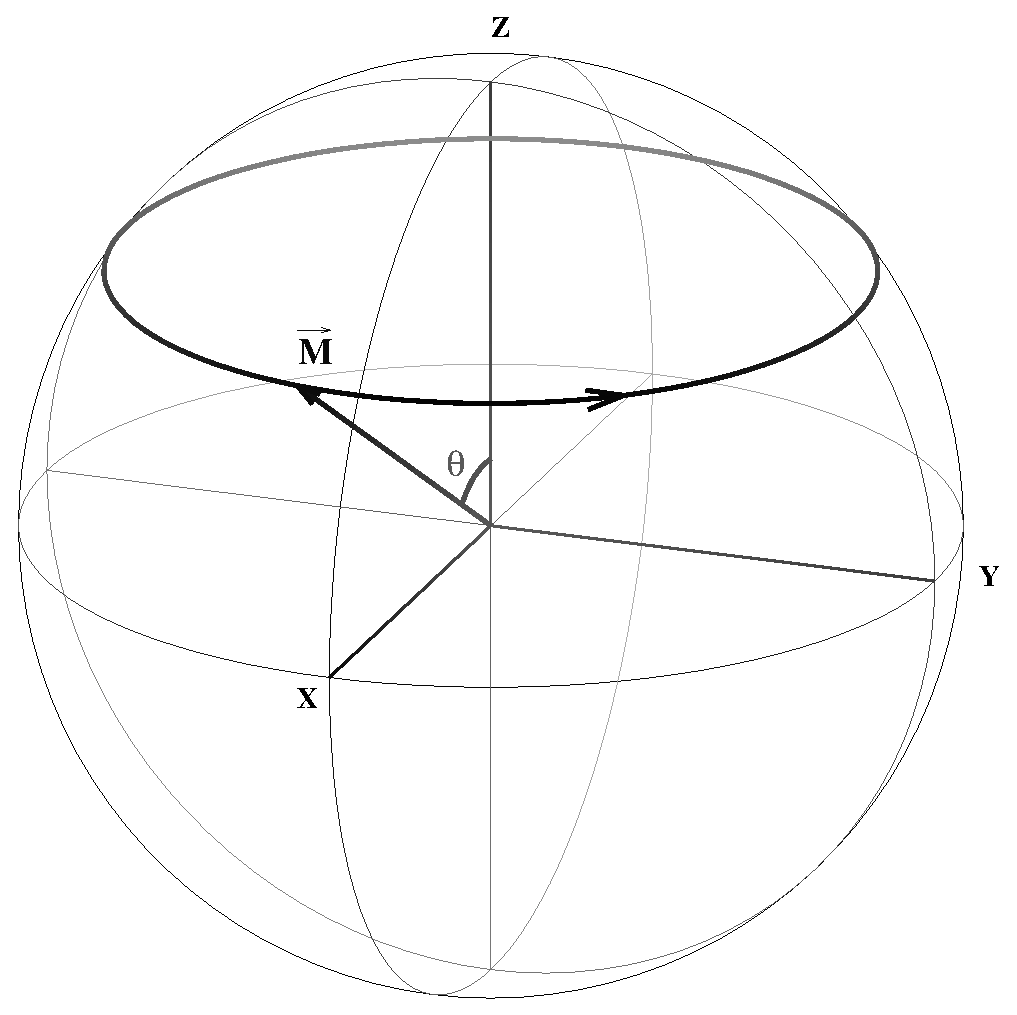
\epsfig{file=larmor.eps,width=4in}
\end{center}
\caption{Précession de Larmor.}
\label{fig:larmor}
\end{figure}

\section{Impulsion, référentiel tournant}
\label{sec:rf}
Le processus qui conduit de l'état d'équilibre $\aimzerovec$ de $\aimvec$
à un état excité résulte de l'action
d'un champ magnétique créé par un courant alternatif sinusoïdal de radiofréquence,
supposé aligné avec l'axe $Ox$ et égal à
\begin{equation}
\bunvect =
2\bunmax \cos(\omrf t+\phi) \ivec
\end{equation}

La pulsation $\omrf$ du champ variable $\bunvect$
est a priori quelconque.
L'angle $\phi$ est appelé la phase de l'impulsion.

De fait, et par la vertu des équations de Maxwell, le champ variable
$\bunvect$ est associé à un champ électrique variable.
L'association de ces deux champs constitue ce qui jusqu'à présent
était désigné sous le terme un peu vague d'OEM excitatrice.
Le fait est que seule la composante magnétique de cette onde
interagit avec les spins nucléaires.
L'interaction de l'OEM avec le système étudié peut donc légitimement
être étudiée comme étant restreinte à la seule action de la composante magnétique
de l'onde excitatrice.
Le champ de radiofréquence est créé par les bobines (dont la géométrie
réelle peut être très éloignée de l'idée de ce que l'on peut se faire d'une bobine,
voir figure \ref{fig:coil})
qui entourent l'échantillon et qui servent à la fois à recueillir les variations
de l'aimantation de l'échantillon sous forme de force électromotrice induite,
mais aussi à exciter l'échantillon lorsqu'elles sont parcourues par
un courant alternatif sinusoïdal de fréquence $\omrf/2\pi$.

\begin{figure}[hbt]
\begin{center}
\begin{pspicture}(-2.5,-2)(2.5,4.5)
\SpecialCoor
\psline(-0.5,4)(-0.5,-1.5)
\psarc(0,-1.5){0.5}{180}{0}
\psline(0.5,4)(0.5,-1.5)
\psellipse(0,1.5)(0.5,0.25)
\psellipse(0,4)(0.5,0.25)
\psline(-2.5,0)(2.5,0)
\psline(0,0.1)(0,-0.1)
\uput[135](0,0){$O$}
\psset{linewidth=0.05}
\psline(-2.5,-1)(-1.5,-1)
\psline{->}(-2.5,-1)(-1.5,-1)
\rput(-1,0){
\pscurve(-0.5,-1)(-0.3,-1)(0,-0.9)(0.2,0)(0,1)(-0.2,0)(0,-0.9)(0.3,-1)(0.5,-1)
}
\psline(-0.5,-1)(0.5,-1)
\rput(1,0){
\pscurve(-0.5,-1)(-0.3,-1)(0,-0.9)(0.2,0)(0,1)(-0.2,0)(0,-0.9)(0.3,-1)(0.5,-1)
}
\psline(1.5,-1)(2.5,-1)
\psline{->}(0,0)(2,0)
\uput[90](2,0){$\bunvect$}
\uput[-90](-1.5,-1){$\boldsymbol{I(t)}$}
\psline{->}(0,0)(0,3)
\uput[90](0,3){$\bzerovec$}
\end{pspicture}
\caption{\label{fig:coil}
% \small Création du champ excitateur $\bunvect$.}
\small Création du champ excitateur.}
\end{center}
\end{figure}

Il est commode de considérer $\bunvect$ comme la
superposition de deux champs magnétiques tournants
$\bunvecplus$ et $\bunvecmoins$ tels que :
\begin{eqnarray}
\bunvecplus & = &
\bunmax\cos(\omrf t + \phi) \ivec +
\bunmax\sin(\omrf t + \phi) \jvec \\
\bunvecmoins & = &
\bunmax\cos(\omrf t + \phi) \ivec -
\bunmax\sin(\omrf t + \phi) \jvec
\end{eqnarray}

Cette décomposition est la même que celle introduite lorsqu'il est dit
que la lumière polarisée linéairement peut être considérée comme
la superposition de lumières polarisées circulairement à droite
et à gauche.

Les vecteurs $\bunvecplus$ et $\bunvecmoins$
tournent respectivement dans le plan $xOy$ aux pulsations $+\omrf$ et
$-\omrf$.
Il suffit d'analyser l'action d'un seul de ces deux champs,
$\bunvecplus$ par exemple,
car un seul des deux exerce une influence sur l'aimantation
$\aimvec$ (voir ci-dessous).
Pour la commodité nous écrirons :
\begin{equation}
\label{eqn:bunvect}
\bunvect =
(\bunmax\cos(\omrf t + \phi)\ivec + \bunmax\sin(\omrf t + \phi)\jvec)
\end{equation}

L'équation \ref{eqn:bloch0} devient
\begin{equation}
\label{eqn:blochrf0}
\derivt{\aimvec} = \gamma \aimvec \wedge (\bzerovec + \bunvect)
\end{equation}

Si on définit
\begin{equation}
\omuns = -\gamma \bunmax
\end{equation}

l'équation \ref{eqn:blochrf0} devient
\begin{equation}
\label{eqn:blochrf1}
\derivt{\aimvec} =
(\omega_0 \kvec + \omuns(\cos(\omrf t + \phi) \ivec + \sin(\omrf t + \phi) \jvec))
\wedge \aimvec
\end{equation}

La résolution de cette équation où le champ magnétique dépend du temps
est facilitée si on change les axes de projection $Ox$, $Oy$
et $Oz$ de façon à rendre le second membre de l'équation \ref{eqn:blochrf1} indépendant
du temps.
Cela est réalisé en choisissant d'observer $\aimvec$ dans un repère tournant
autour de l'axe $Oz$ à la
pulsation $\omrf$ de la composante du champ magnétique excitateur
qui tourne dans le même sens que $\aimvec$ (figure \ref{fig:refer}).
Dans ce repère d'observation, le champ magnétique $\bunvect$
(ou plus exactement la composante tournante retenue) paraîtra immobile.
Le repère (ou référentiel) tournant aura pour axes $OX$, $OY$ et $OZ$,
portant respectivement les vecteurs unitaires
$\iprimvec$, $\jprimvec$ et $\kprimvec$.
Ces vecteurs sont choisis de façon à coïncider avec
$\ivec$, $\jvec$ et $\kvec$
à l'instant $t$ = 0 de l'établissement du champ $\bunvect$.
Les axes $Oz$ et $OZ$ restant en permanence confondus,
on a : $\kvec = \kprimvec$.

\begin{figure}[hbt]
\begin{center}
\begin{pspicture}(-4,-1)(4,4)
\SpecialCoor
\psline{->}(-4,0)(4,0)
\uput[-90](4,0){$x$}
\psline{->}(0,-1)(0,4)
\uput[180](0,4){$y$}
\uput{7pt}[-120](0,0){$O$}
\psline{->}(0.5;-150)(4;30)
\uput[30](4;30){$X$}
\psline{->}(0.5;-60)(4;120)
\uput[120](4;120){$Y$}
\pscircle*(-3,1){0.02}
\pscircle(-3,1){0.2}
\psset{linewidth=1.2pt}
\psline{->}(0,0)(2;0)
\uput[-90](2;0){$\ivec$}
\psline{->}(0,0)(2;90)
\uput[180](2;90){$\jvec$}
\psline{->}(0,0)(2;30)
\uput[120](2;30){$\iprimvec$}
\psline{->}(0,0)(2;30)
\uput[-150](2;120){$\jprimvec$}
\uput{8pt}[90](-3,1){$\kvec=\kprimvec$}
\psset{linewidth=0.08pt}
\psarc[arcsepB=1.2pt]{->}(0,0){2.5}{0}{30}
\uput[15](2.5;15){$\omrft$}
\end{pspicture}
\caption{\label{fig:refer}
\small Référentiel du laboratoire et référentiel tournant.}
\end{center}
\end{figure}

Ce changement de repère apporte le résultat souhaité (annexe \ref{chap:refer} pour le détail des
calculs), à savoir de faire disparaître les termes dépendants du temps.
L'équation \ref{eqn:blochrf1} devient identique dans sa forme à l'équation
\ref{eqn:bloch1}.
\begin{equation}
\label{eqn:blochrf2}
\derivt{\aimvec} = \omveceff \wedge \aimvec
\end{equation}

L'axe et la pulsation de la précession de Larmor dans le référentiel tournant sont donnés
par la direction et la mesure algébrique de $\omveceff$ (figure \ref{fig:effectif}) :
\begin{equation}
\omveceff =
(\omega_0 - \omrf) \kvec + \omuns \uvec = \omzerovec + \omunvec
\end{equation}
où le vecteur unitaire $\uvec$ est fixe dans le repère tournant
et reflète la phase de l'impulsion :
\begin{equation}
\uvec =
\cos\phi\iprimvec +
\sin\phi\jprimvec
\end{equation}

\begin{figure}[hbt]
\begin{center}
\begin{pspicture}(-1,-1)(4,5)
\SpecialCoor
\uput{10pt}[-165](0,0){$O$}
\psline{->}(1;170)(5;-10)
\uput[0](5;-10){$X$}
\psline{->}(0,0)(1.5;-10)
\uput[-90](1.5;-10){$\iprimvec$}
\psline{->}(1;-140)(5;40)
\uput[40](5;40){$Y$}
\psline{->}(0,0)(1.5;40)
\uput{4pt}[-20](1.5;40){$\jprimvec$}
\psline{->}(1;-90)(5;90)
\uput[180](5;90){$Z$}
\psline{->}(0,0)(1.5;90)
\uput[180](1.5;90){$\kprimvec$}
\psset{linewidth=1.2pt}
\psline{->}(0,0)(2,0.5)
\uput[0](2,0.5){$\omunvec$}
\psline{->}(0,0)(!1.5 2 mul 2 2 mul 0.5 0.5 mul add sqrt div 1.5 0.5 mul 2 2 mul 0.5 0.5 mul add sqrt div)
\uput[-120](!1.5 2 mul 2 2 mul 0.5 0.5 mul add sqrt div 1.5 0.5 mul 2 2 mul 0.5 0.5 mul add sqrt div){$\uvec$}
\psline{->}(0,0)(2,3.5)
\uput[60](2,3.5){$\omveceff=-\gamma \bveceff$}
\psline{->}(0,0)(0,3)
\uput[135](0,3){$\omzerovec$}
\psline[linestyle=dashed,dash=3pt 3pt](2,0.5)(2,3.5)
\psline[linestyle=dashed,dash=3pt 3pt](0,3)(2,3.5)
\psset{linewidth=0.8pt}
\psarc{->}(0,0){1.75}{-10}{14.03}
\uput[2](1.75;2){$\phi$}
\end{pspicture}
\caption{\label{fig:effectif}
\small Action d'une impulsion de RF, vue dans le référentiel tournant.}
\end{center}
\end{figure}

Le champ de radiofréquence créé par les bobines excitatrices est donc
capable de faire tourner l'aimantation macroscopique autour d'un axe
lié au référentiel tournant.
La précession de Larmor dans le référentiel tournant est
amène l'aimantation de l'échantillon
hors de sa position d'équilibre.
Ce paragraphe offre une description beaucoup plus détaillée de ce qui est communément
traduit par la formule "l'aimantation s'est écartée de sa position d'équilibre car
l'échantillon a absorbé l'énergie fournie par le champ excitateur".

\section{Impulsion en résonance et hors résonance}
Dans ce paragraphe l'évolution de $\aimvec$ dans le référentiel tournant est analysé dans
différents cas de figure :
\begin{itemize}
\item $\bunvec$ est appliqué en résonance, c'est-à-dire que la fréquence de l'excitation
est exactement égale à la fréquence de résonance des noyaux considérés :
$\omrf = \omega_0$,
\item $\bunvec$ est "légèrement" hors résonance,
\item $\bunvec$ est "complètement" hors résonance.
\end{itemize}

Si la fréquence du champ $\bunvec$ est exactement égale à la fréquence de résonance des
noyau alors $\omveceff = \omunvec$.
Dès que $\bun$ n'est plus nul, $\aimvec$ tourne autour de
l'axe horizontal porté par le vecteur $\uvec$ à la fréquence $\omuns/2\pi$.
Si l'angle de phase $\phi$ est nul, l'axe de rotation de $\aimvec$ est l'axe $OX$
(Figure \ref{fig:onres}).

\begin{figure}[hbt]
\begin{center}
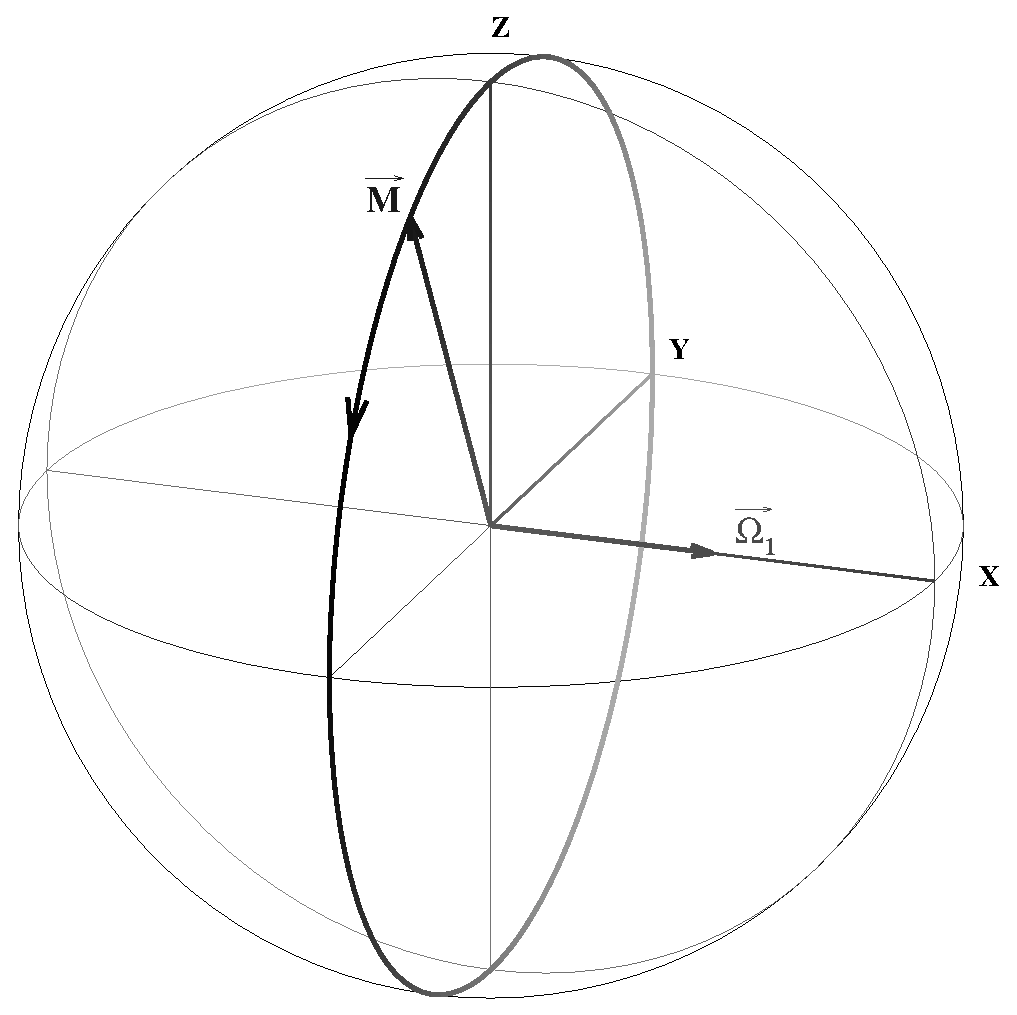
\epsfig{file=off0.eps,width=4in}
\end{center}
\caption{Excitation en résonance.}
\label{fig:onres}
\end{figure}

L'angle $\theta$ de la rotation de $\aimvec$ causée par l'application du champ $\bunvec$
pendant une durée $T$ vaut $\omuns T$.
Cet angle est aussi appelé angle de nutation.
S'il est égal à $\pi/2$, l'aimantation initialement dirigée selon l'axe $OZ$
devient $-\aimzeros\jprimvec$.
Le signe des angles de rotation résulte d'un certain nombre de conventions et
nous adopterons celle qui consiste à utiliser la règle du tire-bouchon :
Le tire-bouchon étant placé sur l'axe $OX$, il faut amener $\aimvec$ en direction
de l'axe $OY$ dans le sens des $Y$ négatifs pour faire avancer la vrille vers les $X$
positifs si l'angle $\theta$ est positif.

Pratiquement, les valeurs de la phase les plus utilisées sur un spectromètre
sont 0, $\pi/2$, $\pi$, $3\pi/2$.
Les impulsions correspondantes seront notées successivement $\theta_x$,
$\theta_y$, $\theta_{-x}$, $\theta_{-y}$ pour en rappeler
à la fois l'angle et l'axe de rotation.
L'effet de ces impulsions est donnée par le tableau \ref{tab:phase}.

\begin{table}
\caption{Action d'une impulsion de RF sur l'aimantation d'équilibre}
\label{tab:phase}
\begin{center}
\begin{tabular}[hbt]{ccc}
\hline
Impulsion & Phase($\phi$) & $\aimvec$ final \\ \hline
$\theta_{x}$  & $0$      & $-\aimzeros\sin\theta\jprimvec + \aimzeros\cos\theta\kprimvec$ \\
$\theta_{y}$  & $\pi/2$  & $+\aimzeros\sin\theta\iprimvec + \aimzeros\cos\theta\kprimvec$ \\
$\theta_{-x}$ & $\pi$    & $+\aimzeros\sin\theta\jprimvec + \aimzeros\cos\theta\kprimvec$ \\
$\theta_{-y}$ & $-\pi/2$ & $-\aimzeros\sin\theta\iprimvec + \aimzeros\cos\theta\kprimvec$ \\
\hline
\end{tabular}
\end{center}
\end{table}
Le vecteur $\aimvec$ à la fin de l'impulsion se réécrit de façon plus générale sous la forme :
\begin{equation}
\label{eqn:pulseaction}
\aimvec = \aimzeros \sin\theta (\cos(\phi-\pi/2)\iprimvec +
\sin(\phi-\pi/2)\jprimvec) + \aimzeros\cos\theta\kprimvec
\end{equation}
L'angle que fait la composante horizontale de $\aimvec$ avec le vecteur $\iprimvec$
est égal à la phase de l'impulsion, à $\pi/2$ près.

Des noyaux hors résonance sont caractérisés par leur "décalage" (offset)
à savoir la pulsation $\omzeros = \omega_0 - \omrf$.
Ils subissent en première approximation les mêmes actions dues au
champ $\bunvec$ si la condition $|\omzeros| << \omuns$ est vérifiée.
Cela nécessite un champ magnétique $\bunvec$ suffisamment intense pour
que $\omuns/2\pi$ soit grand par rapport à l'écart
entre la fréquence de résonance des noyaux et la fréquence des impulsions.
Plus $\bunvec$ sera intense et plus l'excitation des différents noyaux (de même nature)
de l'échantillon sera uniforme.
En conséquence les impulsions doivent être les plus courtes possible pour un
angle de rotation donné.
La durée des impulsions est généralement inférieure à 10 $\mu$s
pour un angle de $\pi/2$.

\begin{figure}[hbt]
\begin{center}
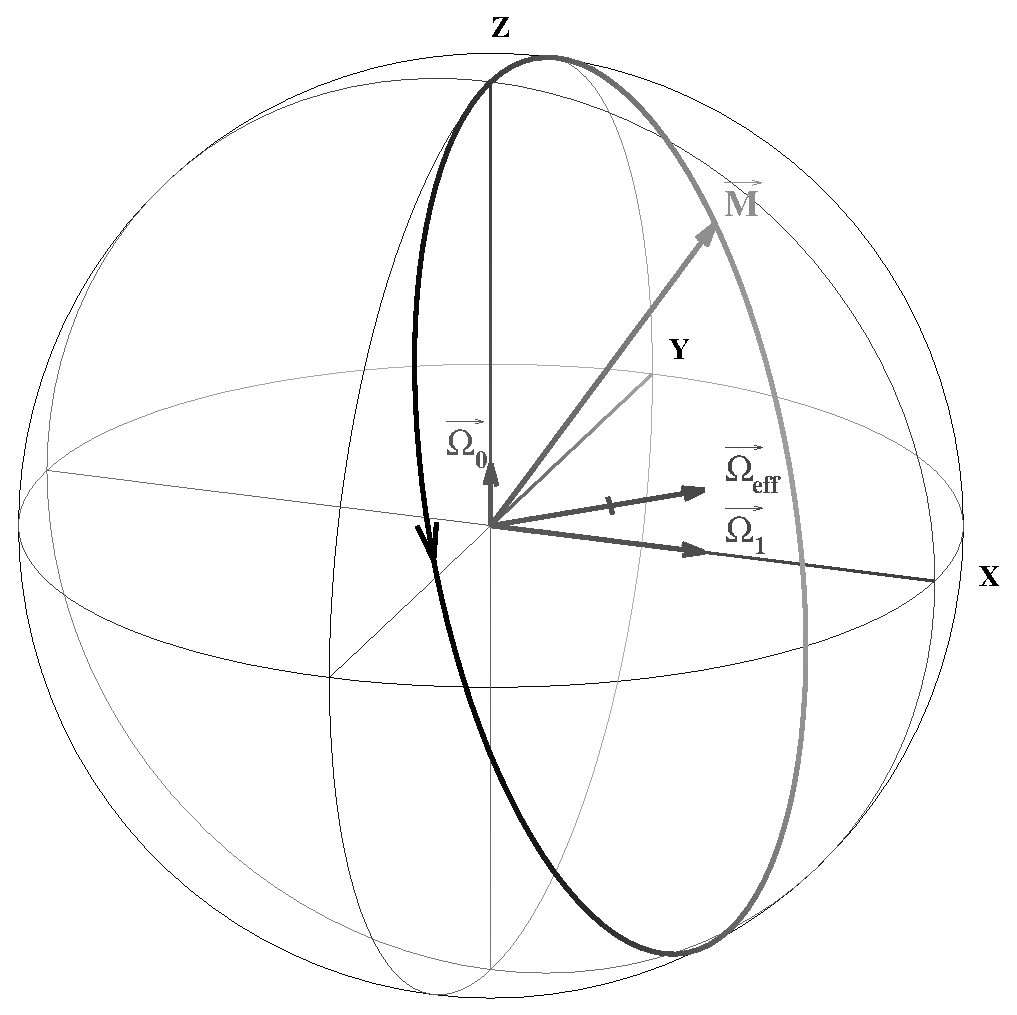
\epsfig{file=off1.eps,width=4in}
\end{center}
\caption{Excitation légèrement hors résonance.}
\label{fig:offres}
\end{figure}

Si $|\omzeros|$
 est de l'ordre de grandeur de $\omuns$
l'axe de rotation fait un angle $\theta$ significatif avec le plan
$XOY$ (Figure \ref{fig:offres}) :
\begin{equation}
\tan \theta =  \frac{\omzeros}{\omuns}
\end{equation}

La pulsation de rotation est la norme du vecteur $\omveceff$ :
\begin{equation}
\omeff = \sqrt{\omzeros^2 + \omuns^2}
\end{equation}
Dans le cas général la rotation de $\aimvec$ à partir de sa position d'équilibre
ne se fait plus exclusivement dans un plan vertical.

Si $\omuns$ est faible devant $\omzeros$,
les noyaux ne subissent pratiquement pas l'influence du champ de
radiofréquence, car ce dernier est appliqué très loin de la résonance
(Figure \ref{fig:veryoffres}).

Les noyaux de nature différente ont des gammes de fréquence de résonance
suffisamment éloignées les unes des autres pour que, par exemple, il soit impossible
d'exciter simultanément les protons et les noyaux de $^{13}$C avec une seule
impulsion.
Nous avons souligné qu'un champ magnétique linéaire $\bunvec$ de pulsation $\omrf$
résulte de la superposition de deux champs tournants de pulsation $+\omrf$ et $-\omrf$.
Dans les conditions usuelles où $\omega_0$ et $\omrf$ sont très proches,
$+\omrf$ et $-\omrf$ sont nécessairement très
éloignées.
Cela justifie le fait qu'une seule composante
circulaire de $\bunvec$ soit prise en compte dans les calculs.

\begin{figure}[hbt]
\begin{center}
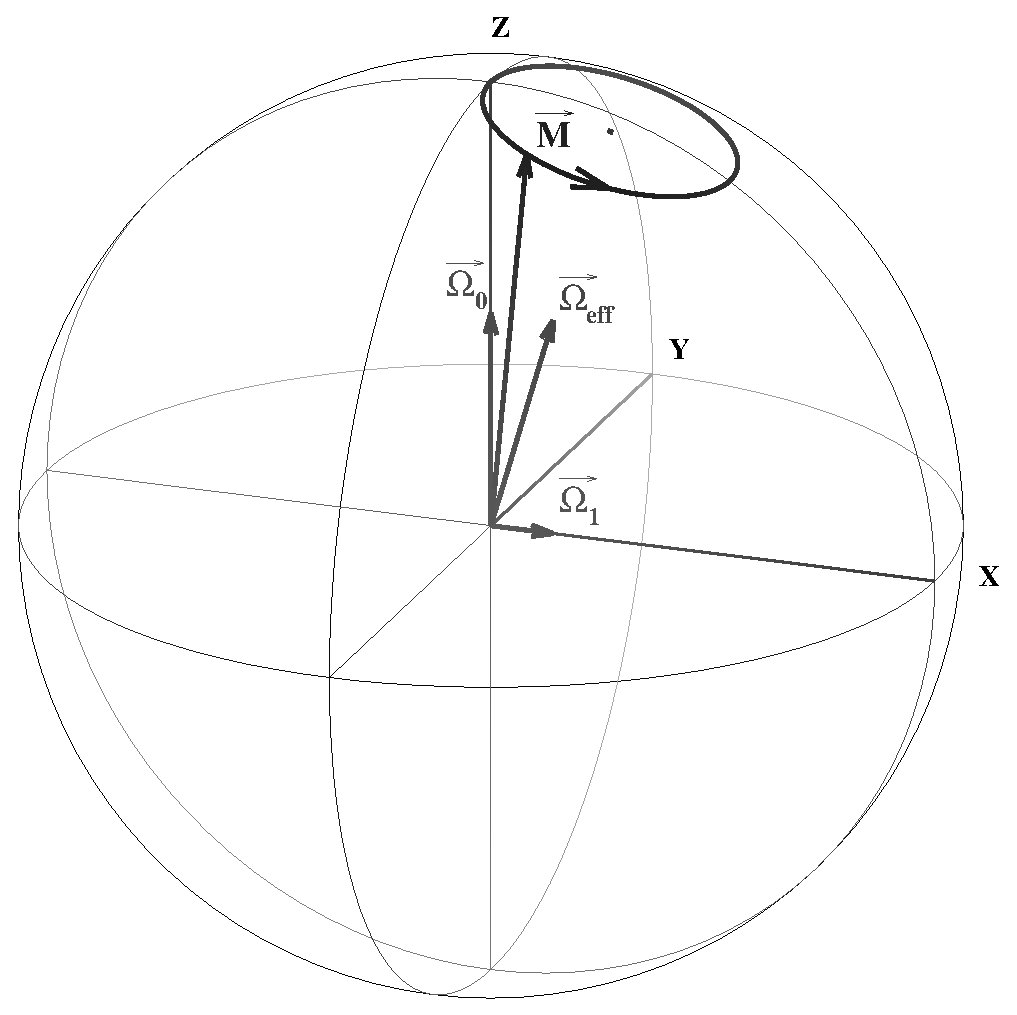
\epsfig{file=off2.eps,width=4in}
\end{center}
\caption{Excitation très loin de la résonance.}
\label{fig:veryoffres}
\end{figure}

\section{Après l'impulsion}
Lorsque $\bunvec$ redevient nul, le vecteur $\aimvec$ ne subit plus que l'action de
$\bzerovec$, et son mouvement dans le référentiel du laboratoire est le mouvement
de précession de Larmor de pulsation $\omega_0$ décrit au paragraphe \ref{sec:larmor}.

Sachant que le sens de rotation du référentiel tournant est celui de la
rotation libre (de Larmor) de $\aimvec$,
ce dernier tourne par rapport au référentiel tournant à la pulsation $\omzeros$
\begin{equation}
\omzeros = \omega_0 - \omrf
\end{equation}
sachant que le référentiel tournant tourne autour du référentiel du laboratoire
à la pulsation $\omrf$.

On constate que la description du mouvement de l'aimantation
macroscopique se résume (hors relaxation) à de simples rotations
si elle est effectuée dans le référentiel tournant.
Cette simplicité est liée au fait que dans ce référentiel tout
se passe comme $\aimvec$ n'était soumis qu'à des champs magnétiques constants.

\section{Relaxation}
Le traitement mécanique de l'évolution de l'aimantation d'un ensemble de noyaux tel
qu'il vient d'être traité néglige complètement l'effet de la relaxation, c'est à dire de
l'ensemble des phénomènes qui tendent à ramener $\aimvec$ à sa position initiale dès qu'elle
s'en écarte.
Il est commode pour étudier leur effet de se placer dans le référentiel
tournant à pulsation $\omzeros$, référentiel où $\aimvec$ paraît immobile en
l'absence de champ magnétique $\bunvec$ et de phénomènes de relaxation.
Sauf si les noyaux étudiés sont en résonance, il ne s'agit pas du référentiel tournant
au sens où il a été défini au paragraphe précédent.
Dans le référentiel d'étude, $\aimvec$ évolue en restant dans le plan $\Pi$ défini par $\aimvec$
et $\bzerovec$.

A chaque instant $t$ la variation des composantes $\aimzs$ et $\aimxys$ est proportionnelle à l'écart
entre leur valeur au temps $t$ et leur valeur d'équilibre :
\begin{eqnarray}
\label{eqn:t1}
\derivt{\aimzs} & = & -\frac{\aimzs - \aimzerozs}{T_1} \\
\label{eqn:t2}
\derivt{\aimxys} & = & -\frac{\aimxys - \aimzeroxys}{T_2}
\end{eqnarray}
Avec
\begin{eqnarray}
\aimzerozs & = & \aimzeros \\
\aimzeroxys & = & 0
\end{eqnarray}

$T_1$ et $T_2$ sont appelés temps de relaxation longitudinal (ou spin-réseau)
et transversal (ou spin-spin).
Ces deux grandeurs sont hautement dépendantes de la nature du noyau
considéré, de l'état de l'échantillon (solide ou liquide), de la température, de
l'environnement moléculaire...

Le mouvement de $\aimvec$ dans le plan $\Pi$ se déduit en résolvant les équations
différentielles \ref{eqn:t1} et \ref{eqn:t2}.
La relaxation transversale "amortit" $\aimxys$
suivant la loi :
\begin{equation}
\aimxys (t) = \aimxys (t=0) . \exp \left( -\frac{t}{T_2} \right)
\end{equation}

Cet affaiblissement de $\aimxy$ est un phénomène à caractère irréversible,
contrairement à celui provoqué par les inhomogénéités de $\bzerovec$,
qui peuvent être corrigées par écho de spin (voir section \ref{sec:echodespin}).
Les imperfections de $\bzerovec$ font que des sous-populations de noyaux précessent à des
fréquences légèrement différentes les unes des autres, la somme vectorielles de leurs
moments magnétiques tend alors à s'annuler.

La figure \ref{fig:isochrom} montre l'aimantation résultante $\aimvec$ issue de cinq zones
de l'échantillon où $\bzero$ s'échelonne régulièrement entre une valeur minimale
et une valeur maximale (il s'agit plus d'une caricature que d'une situation réaliste).
Immédiatement après l'impulsion, les aimantations des cinq zones sont toutes alignées
sur un axe du plan transversal (diagramme de gauche).
Après une première période d'évolution, chaque aimantation élémentaire aura
tourné d'une quantité proportionnelle à $\bzeros$, certaines tournent
donc plus vite que d'autres (diagramme du centre).
Leur somme vectorielle aura en conséquence une norme $\aims$ plus faible que 
celle de l'aimantation totale initiale, et ceci même en l'absence de relaxation.
L'affaiblissement de $\aims$ est encore plus net après une seconde
période d'évolution (diagramme de droite).

\begin{figure}[hbt]
\begin{center}
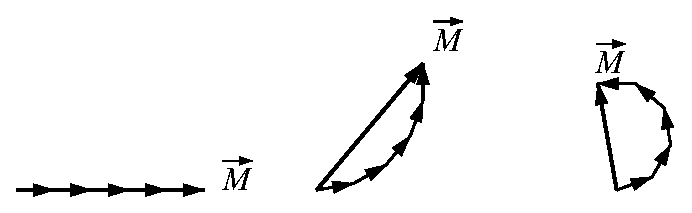
\epsfig{file=isochrom.eps,width=4in}
\end{center}
\caption{Effet de l'inhomogénéité de $\bzero$ sur l'évolution de l'aimantation transversale.}
\label{fig:isochrom}
\end{figure}

Expérimentalement on observe un affaiblissement de $\aimxys$ qui peut s'écrire
en première approximation par :
\begin{equation}
\aimxys (t) = \aimxys (t=0) . \exp \left( -\frac{t}{T_2^*} \right)
\end{equation}
où $T_2^*$ est le temps de relaxation transversal apparent, inférieur à $T_2$.

Indépendamment de $\aimxys$, $\aimzs$ évolue selon
\begin{equation}
\aimzs(t) = \aimzeros + (\aimzs (t=0) - \aimzeros)\exp \left( -\frac{t}{T_1} \right)
\end{equation}

Après une impulsion d'angle $\pi/2$, la composante longitudinale de $\aimvec$
est nulle et donc
\begin{eqnarray}
\label{eqn:relaxlong}
\aimzs(t) & = & \aimzeros \left( 1 - \exp \left( -\frac{t}{T_1} \right) \right) \\
\label{eqn:relaxtrans}
\aimxys(t) & = & \aimzeros \exp \left( -\frac{t}{T_2^*} \right)
\end{eqnarray}

Dans cette situation, la variation de $\aimzs$ et $\aimxys$ en fonction du temps 
est tracée figure \ref{fig:relax}.
En règle générale $T_2 \le T_1$.

\begin{figure}[hbt]
\begin{center}
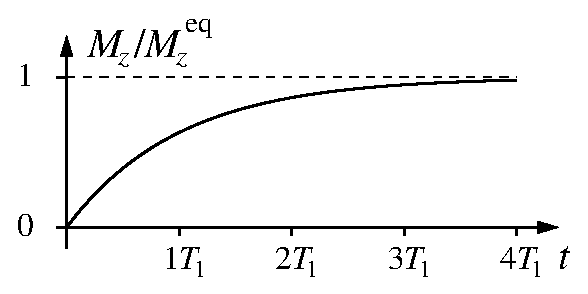
\epsfig{file=relaxlong.eps,width=2.5in}
\hspace{0.25in}
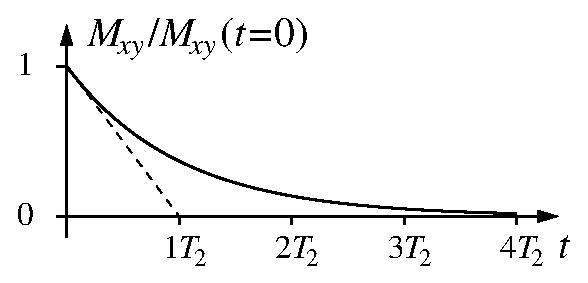
\epsfig{file=relaxtrans.eps,width=2.5in}
\end{center}
\caption{Relaxation longitudinale et transversale.}
\label{fig:relax}
\end{figure}

L'ordre de grandeur de $T_1$ et $T_2$ varie dans une gamme très large.
Il n'y a pas lieu de tenir compte de la relaxation pendant une impulsion de radio-fréquence
si $1/\omuns$ est faible par rapport aux temps de relaxation.
Les impulsions de grande durée et de faible intensité, voient leur efficacité modifiée par la
relaxation, donnant lieu au phénomène de saturation, qui ne sera pas étudié dans ce paragraphe.

Les expressions de $\aimxs (t)$ et de $\aimys (t)$ obtenues au paragraphe \ref{sec:larmor}
par résolution de l'équation du mouvement de $\aimvec$ dans le champ
$\bzerovec$ sont modifiées par la relaxation :
\begin{eqnarray}
\aimxs (t) & = & A\cos(\omega_0 t + \phi) \exp \left( -\frac{t}{T_2^*} \right) \\
\aimys (t) & = & A\sin(\omega_0 t + \phi) \exp \left( -\frac{t}{T_2^*} \right)
\end{eqnarray}

Le moment magnétique total d'un ensemble de noyaux est décrit d'une façon très
générale en tenant compte de l'action de $\bzerovec$, de l'action du champ de
radio-fréquence et des processus de relaxation.
Les équations différentielles qui résument l'effet de toutes ces
interactions sont désignées sous le nom d'équations de Bloch.

\section{Équations de Bloch}
\label{sec:eqnbloch}
Dans le référentiel tournant, l'équation \ref{eqn:blochrf2} décrit l'évolution
de $\aimvec$ sous l'action de $\bzerovec$ (modifiée par l'écran électronique)
et du champ de radiofréquence $\bunvec$, mais en l'absence de relaxation.
En considérant que la phase de $\bunvec$ est nulle, 
\begin{equation}
\omveceff = \left| \begin{array}{l}\omuns \\ 0 \\ \omzeros \end{array} \right.
\quad\mbox{et donc}\quad
\aimvec\wedge\omveceff = \left| \begin{array}{l} 
\aimys\omzeros \\ \aimzs\omuns-\aimxs\omzeros \\ -\aimys\omuns \end{array} \right.
\end{equation}
et vu que la relaxation agit aussi pendant l'application du champ $\bunvec$
selon les équations \ref{eqn:t1} et \ref{eqn:t2}, l'équation \ref{eqn:blochrf2}
devient :
\begin{eqnarray}
\derivt{\aimxs} & = & \aimys\omzeros - \frac{1}{T_2}\aimxs \\
\derivt{\aimys} & = & \aimzs\omuns-\aimxs\omzeros - \frac{1}{T_2}\aimys \\
\derivt{\aimzs} & = & -\aimys\omuns - \frac{1}{T_1} (\aimzs-\aimzerozs)
\end{eqnarray}
qui constituent les équations de Bloch.

Dans une expérience de RMN par impulsion et transformation de Fourier
utilisant des impulsions de RF brèves (quelques $\mu$s) par rapport à
$T_1$ et $T_2$ (au moins des ms, voire des secondes),
il est légitime d'ignorer l'effet de la relaxation pendant les impulsions.
La RMN par onde continue s'appuie sur la détection des états d'aimantation
qui correspondent à des solutions (quasi--)stationnaires des équations de Bloch.
Cet aspect de la RMN ne sera pas détaillé ici, sauf dans le cas
d'un champ $\bunvec$ appliqué en résonance ($\omzeros = 0$), car il aboutit
à la saturation de l'aimantation, utilisée pour l'établissement
de l'effet Overhauser nucléaire (section \ref{sec:noe}).
A l'état stationnaire, les coordonnées de $\aimvec$ sont indépendantes
du temps, Ainsi :
\begin{eqnarray}
0 & = & - \frac{1}{T_2}\aimxs \\
0 & = & \aimzs\omuns - \frac{1}{T_2}\aimys \\
0 & = & -\aimys\omuns - \frac{1}{T_1} (\aimzs-\aimzerozs)
\end{eqnarray}
dont la solution est :
\begin{eqnarray}
\aimxs & = & 0 \\
\aimys & = & \frac{\aimzerozs\omuns T_2}{1+\omuns^2 T_1 T_2} \\
\aimzs & = & \frac{\aimzerozs}{1+\omuns^2 T_1 T_2}
\end{eqnarray}

Si $\omuns \gg 1/\sqrt{T_1 T_2}$, alors $\aimzs \ll \aimzerozs$, ce qui
traduit une égalisation des populations des états $\al$ et $\be$ des spins nucléaires,
avec une disparition complète de l'aimantation macroscopique.
